% !TeX program = pdfLaTeX
\documentclass[smallextended]{svjour3}       % onecolumn (second format)
%\documentclass[twocolumn]{svjour3}          % twocolumn
%
\smartqed  % flush right qed marks, e.g. at end of proof
%
\usepackage{amsmath}
\usepackage{graphicx}
\usepackage[utf8]{inputenc}

\usepackage[hyphens]{url} % not crucial - just used below for the URL
\usepackage{hyperref}

%
% \usepackage{mathptmx}      % use Times fonts if available on your TeX system
%
% insert here the call for the packages your document requires
%\usepackage{latexsym}
% etc.
%
% please place your own definitions here and don't use \def but
% \newcommand{}{}
%
% Insert the name of "your journal" with
% \journalname{myjournal}
%

%% load any required packages here



% tightlist command for lists without linebreak
\providecommand{\tightlist}{%
  \setlength{\itemsep}{0pt}\setlength{\parskip}{0pt}}

% From pandoc table feature
\usepackage{longtable,booktabs,array}
\usepackage{calc} % for calculating minipage widths
% Correct order of tables after \paragraph or \subparagraph
\usepackage{etoolbox}
\makeatletter
\patchcmd\longtable{\par}{\if@noskipsec\mbox{}\fi\par}{}{}
\makeatother
% Allow footnotes in longtable head/foot
\IfFileExists{footnotehyper.sty}{\usepackage{footnotehyper}}{\usepackage{footnote}}
\makesavenoteenv{longtable}


\begin{document}


\title{Perdiz arrow points from Caddo burial contexts aid in defining
discrete behavioral regions \thanks{Components of the analytical
workflow were developed and funded by a Preservation Technology and
Training grant (P14AP00138) to RZS from the National Center for
Preservation Technology and Training, as well as grants to RZS from the
Caddo Nation of Oklahoma, National Forests and Grasslands in Texas
(15-PA-11081300-033) and the United States Forest Service
(20-PA-11081300-074). Additional financial and logistical support was
provided by the Heritage Research Center at Stephen F. Austin State
University.} }


    \titlerunning{Perdiz arrow points from Caddo burial contexts}

\author{  Robert Z. Selden 1 \and  John E. Dockall 2 \and  }

    \authorrunning{ Selden and Dockall }

\institute{
        Robert Z. Selden 1 \at
     Heritage Research Center, Stephen F. Austin State University;
Department of Biology, Stephen F. Austin State University; Texas
Archeological Research Laboratory, The University of Texas at Austin;
and Cultural Heritage Department, Jean Monnet University \\
     \email{\href{mailto:zselden@sfasu.edu}{\nolinkurl{zselden@sfasu.edu}}}  %  \\
%             \emph{Present address:} of F. Author  %  if needed
    \and
        John E. Dockall 2 \at
     Stantec, Inc. \\
     \email{\href{mailto:john.dockall@stantec.com}{\nolinkurl{john.dockall@stantec.com}}}  %  \\
%             \emph{Present address:} of F. Author  %  if needed
    \and
    }

\date{Received: date / Accepted: date}
% The correct dates will be entered by the editor


\maketitle

\begin{abstract}
Recent research into Caddo bottle and biface morphology yielded evidence
for two distinct behavioral regions, across which material culture from
Caddo burials expresses significant morphological differences. This
study asks whether Perdiz arrow points from Caddo burials differ across
the same geography, which would extend the pattern of morphological
differences to a third category of Caddo material culture. Perdiz arrow
points collected from the geographies of the northern and southern Caddo
behavioral regions were employed to test the hypothesis that
morphological attributes differ, and are predictable, between the two
communities. The analysis of linear metrics indicated a significant
difference in morphology by behavioral region. Using the linear metrics
combined with the tools of machine learning, a predictive
model---support vector machine---was designed to assess the degree to
which community differences could be predicted, achieving a receiver
operator curve score of 97 percent, and an accuracy score of 94 percent.
The subsequent landmark geometric morphometric analysis identified
significant differences in Perdiz arrow point shape and size between the
behavioral regions---one characterized by a comparatively smaller blade
and larger stem (north), and the other by a comparatively larger blade
and smaller stem (south)---coupled with significant results for
modularity and morphological integration. These findings build directly
upon recent investigations that posited two discrete Caddo behavioral
regions defined on the basis of discernible morphological differences,
which is expanded here to include a third category of Caddo material
culture.
\\
\keywords{
        American Southeast \and
        Caddo \and
        NAGPRA \and
        computational archaeology \and
        archaeoinformatics \and
        machine learning \and
        museum studies \and
        digital humanities \and
        non-Western art history \and
        STEM \and
        STEAM \and
    }


\end{abstract}


\def\spacingset#1{\renewcommand{\baselinestretch}%
{#1}\small\normalsize} \spacingset{1}


\hypertarget{intro}{%
\section{Introduction}\label{intro}}

Perdiz arrow points are considered the epitome of the Late Prehistoric
Toyah lithic assemblage in Texas---which also includes convex end
scrapers or unifaces, prismatic blades, as well as two- and four-beveled
bifacial knives---and are representative of the Late Prehistoric
transition to the Protohistoric \cite{RN9718}. This technological
assemblage is typically attributed to groups of highly mobile bison
hunters, and has been documented across the geographic extent of Texas.
Our present understanding of the Toyah tool kit indicates that it was
successfully implemented in a broad-spectrum of hunting and foraging
lifeways that included not only bison (\emph{Bison bison}), but deer
(\emph{Odocoileus spp.}) and numerous other animal prey species
\cite{RN9718,RN9786}.

The Toyah tool kit has been recognized as a potential contributor to
discussions of Late Prehistoric social and cultural identity. Initially
identified by J. Charles Kelley on the basis of technological and
morphological differences in material culture, the Toyah Phase (CE 1300
- 1700) occurrs between the Protohistoric and the preceding Austin Phase
of the Late Prehistoric Period \cite{RN9719,RN9720}. As noted by Arnn:

\begin{quote}
Toyah represents something of a paradox in which archaeologists have
identified \emph{one archaeological or material culture} in the same
region where historians have documented numerous Native American groups
and significant cultural diversity \cite[47]{RN9718}.
\end{quote}

Stemming from the observations of Kelley, as well as later researchers
who viewed Toyah as a cultural entity, technological origins became a
point of further interest and debate from which two schools of thought
emerged regarding Toyah cultural manifestations: 1) that Toyah
represented the technology of Plains groups moving into Texas following
the bison herds \cite{RN9721,RN9722}, or 2) a technocomplex or suite of
artifacts adopted by multiple groups across Texas as they participated
in bison hunting \cite{RN9008,RN9723,RN9724}. In both interpretations,
primary agency is environmental \cite{RN9718}; either people followed
the bison from elsewhere, or the influx of bison spurred adoption of the
technology among the numerous groups in Texas.

Research by Arnn \cite{RN9718,RN9716,RN5784,RN9717} emphasized aspects
of Toyah social identity, social fields, and agency, as well as the
archaeological visibility of these phenomena. Arnn recognized three
important scales of identity and interaction in his work:
community/band, marriage/linguistic group, and long-distance social
networks \cite{RN9718}. His ideas are important here because they
supplant a simple monocausal environmental explanation of material
culture variability with a multi-causal and scaled concept that includes
social identity.

\hypertarget{perdiz-arrow-points}{%
\subsection{Perdiz arrow points}\label{perdiz-arrow-points}}

Perdiz arrow points generally follow two manufacturing
trajectories---one that enlists flakes, and the other, blade flakes
\cite{RN8999,RN9361,RN9000,RN9364}---and are known to encompass a
greater range of variation in shape and size than most arrow point types
in Texas \cite{RN7795,RN3149}. Lithic tool stone in the ancestral Caddo
area of northeast Texas is relatively sparse \cite[Figure 2]{RN9364},
consists primarily of chert, quartzite, and silicified wood
characteristic of the local geological formations, which may contribute
to local variation in shape and size \cite{RN9364,RN439}. It has been
demonstrated elsewhere that the morphological attributes of Perdiz arrow
points from northeast Texas vary significantly by time, raw material,
and burial context \cite{RN9364}. In outline, Perdiz arrow points
possess a:

\begin{quote}
{[}t{]}riangular blade with edges usually quite straight but sometimes
slightly convex or concave. Shoulders sometimes at right angles to stem
but usually well barbed. Stem contracted, often quite sharp at base, but
may be somewhat rounded. Occasionally, specimen may be worked on one
face only or mainly on one face \ldots{} {[}w{]}orkmanship generally
good, sometimes exceedingly fine with minutely serrated blade edges
\cite[504]{RN5769}.
\end{quote}

A social network analysis of diagnostic artifacts from Historic Caddo
(post-CE 1680) sites in northeast Texas, which included Perdiz arrow
points, demonstrated two spatially discrete behavioral regions based
upon the co-presence of diagnostic types \cite[Figure 12.4]{RN8031}. The
network analysis was limited to Historic Caddo types; however,
Formative/Early Caddo (CE 800 -- 1200) Gahagan bifaces and Caddo bottle
types have been found to express significant morphological differences
across the same spatial extent as the behavioral regions
\cite{RN8074,RN7927,RN8370,RN8312}, extending the prehistoric longevity
for the behavioral regions based on local alterity. Gahagan bifaces from
the ancestral Caddo area also differ significantly in shape, size, and
form compared with those recovered from central Texas sites
\cite{RN8322}, suggesting a second shape boundary between the ancestral
Caddo area and central Texas.

\begin{figure}
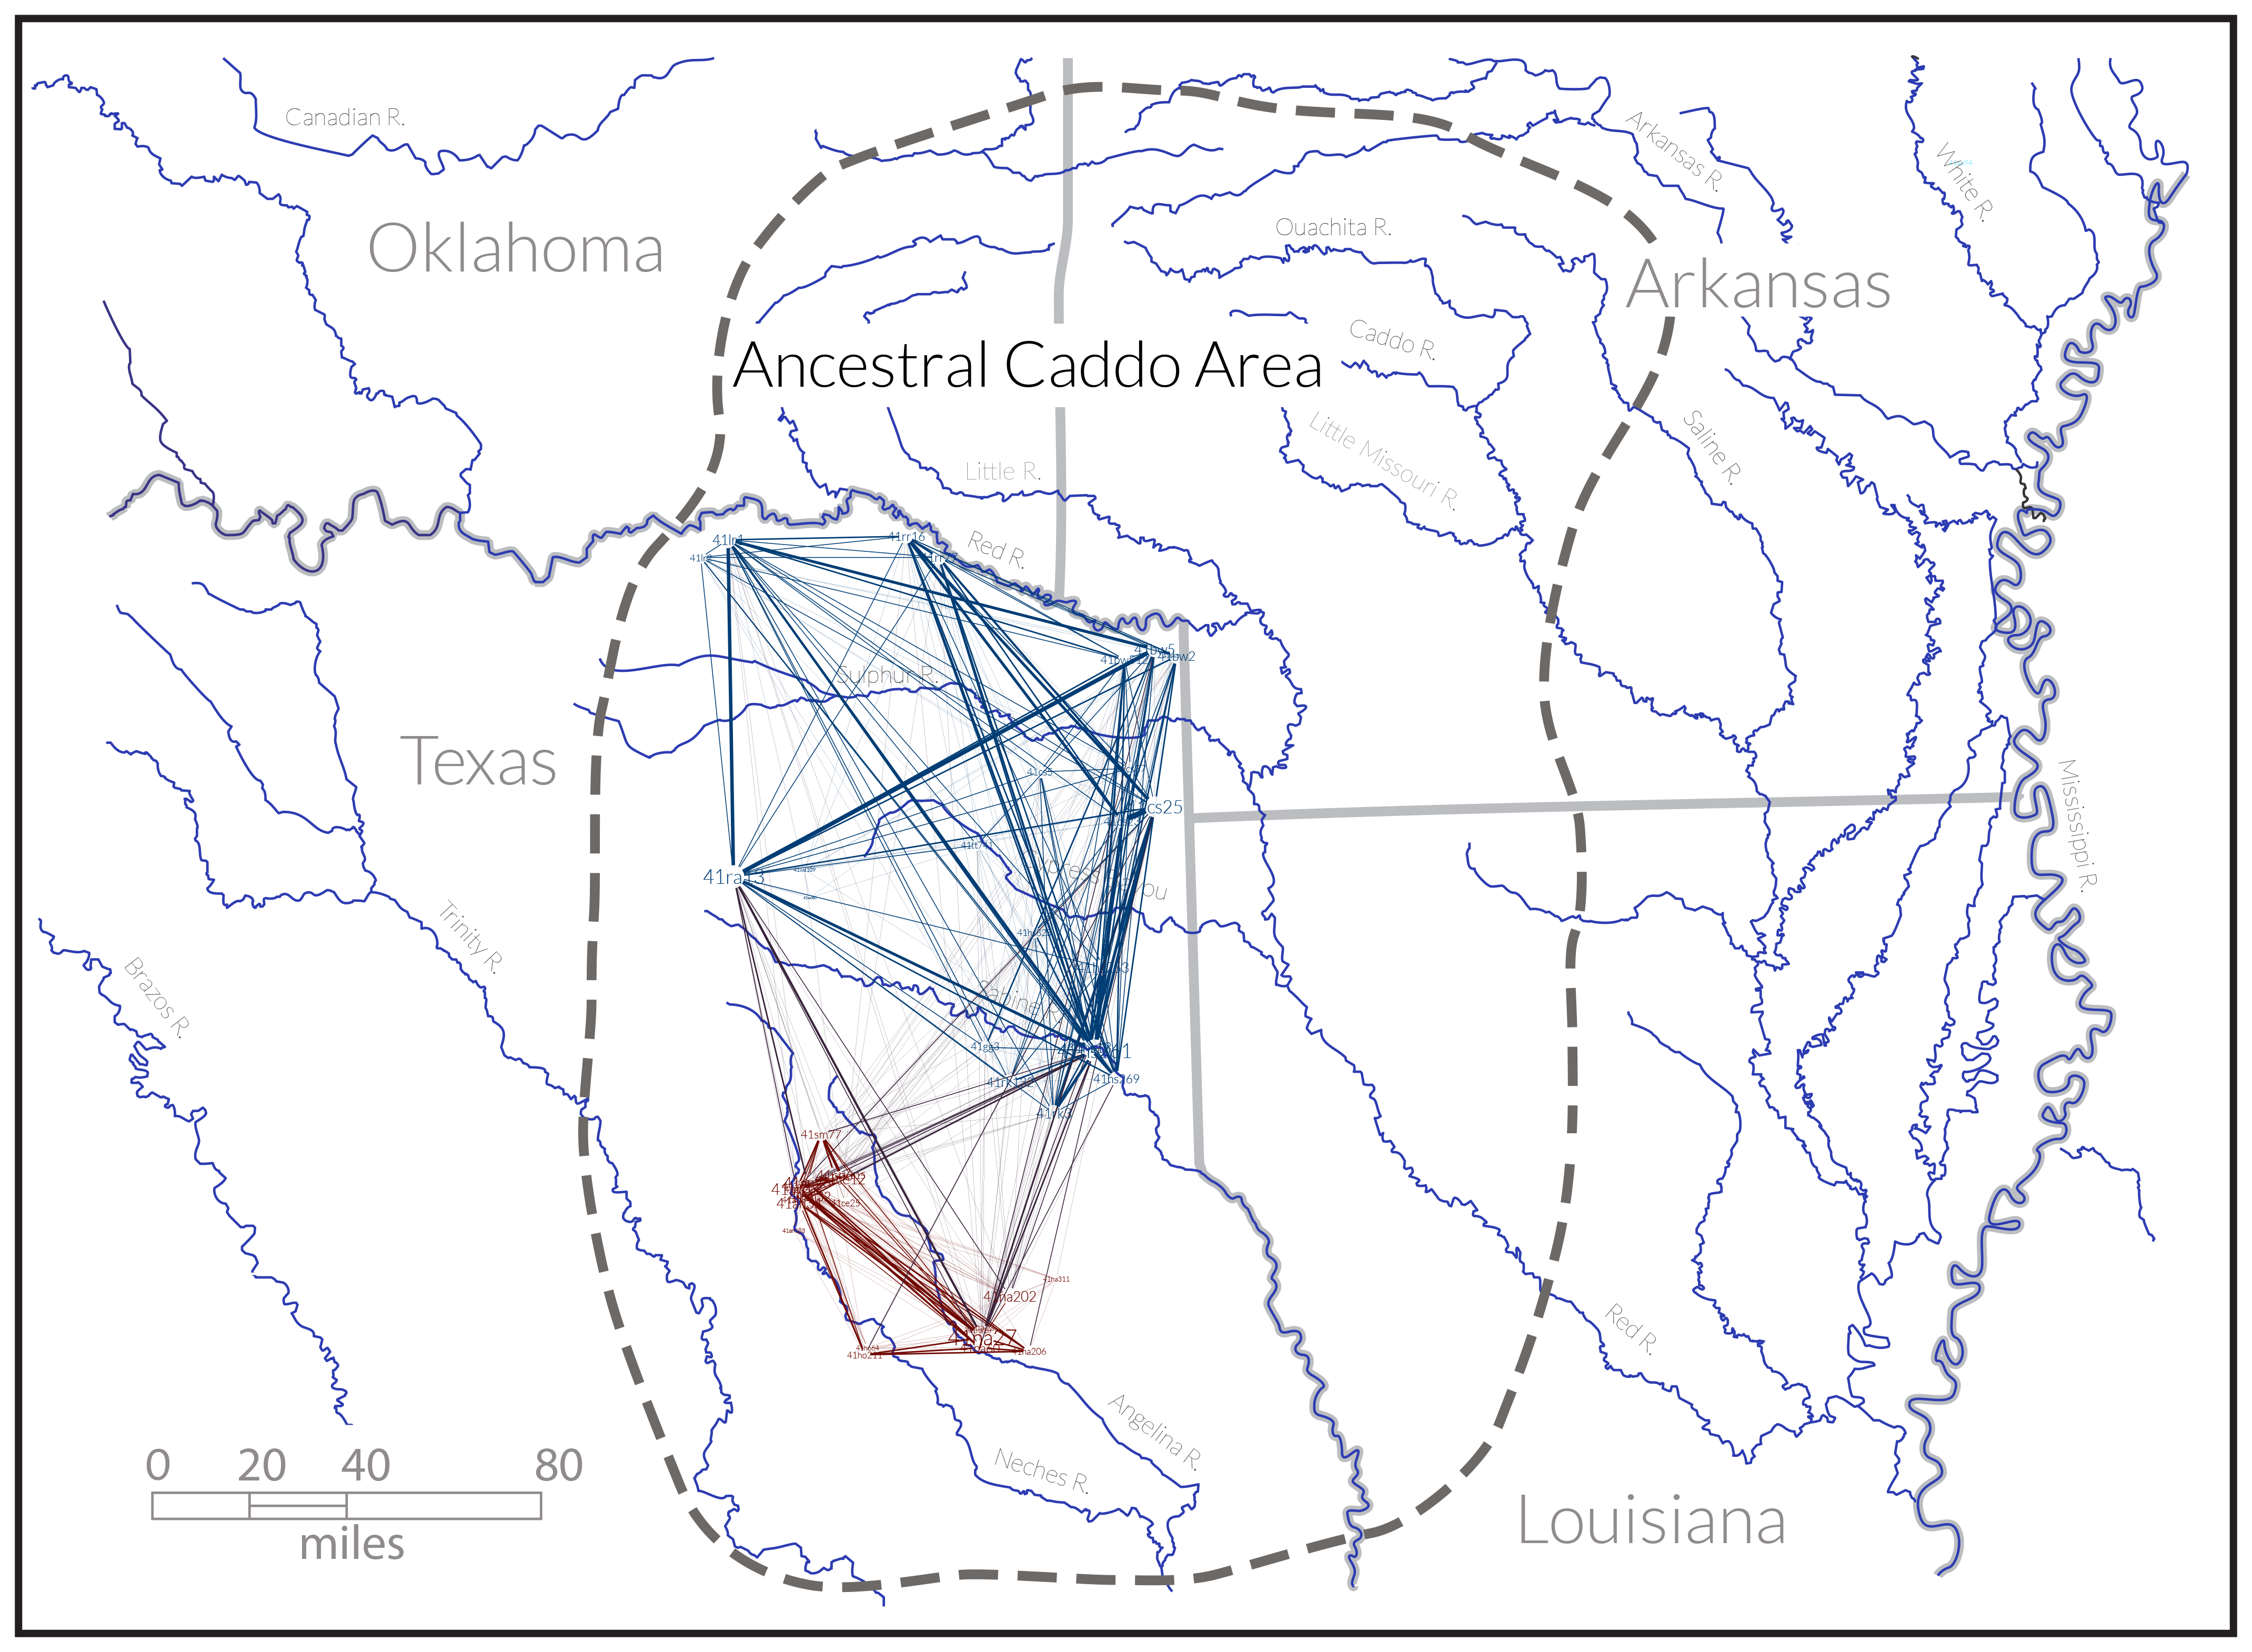
\includegraphics[width=1\linewidth]{ms-figs/figure1} \caption{Location of Caddo sites with Perdiz arrow points used in this study, the extent of the ancestral Caddo area (white), and the Red River basin (blue), Sabine River basin (maroon), and Angelina River basin (brown).}\label{fig:fig1}
\end{figure}

The goal of this exploratory endeavor was to assess whether metrics
collected for Perdiz arrow points support the shape boundary posited in
recent social network and geometric morphometric analyses, to determine
whether linear metrics and shape variables might be useful predictors of
regional membership, and---if so---to identify those morphological
features that articulate with each behavioral region. Should the
analysis yield significant results, it would bolster the argument for at
least two discrete Caddo behavioral regions in northeast Texas; each
empirically defined by discernible morphological differences across
three discrete categories of Caddo material culture (Figure
\ref{fig:fig1}).

\hypertarget{caddo-behavioral-regions}{%
\subsection{Caddo behavioral regions}\label{caddo-behavioral-regions}}

In a June 18, 1937 Works Progress Administration interview with Lillian
Cassaway, Sadie Bedoka---a Caddo-Delaware woman raised with the
Caddo---stated that:

\begin{quote}
Each {[}Caddo{]} clan had its own shape to make its pottery. One clan
never thought of making anything the same pattern of another clan.
\emph{\textbf{You could tell who made the pottery by the shape}}
\cite[395]{RN9357x}.
\end{quote}

General differences in Caddo ceramic forms have been noted elsewhere
\cite{RN5650,RN7162}; however, the study of the Clarence H. Webb
collection was the first to illustrate a significant north-south
geographic shape difference among Hickory Engraved and Smithport Plain
Caddo bottle types \cite{RN8370}. That exploratory aperçu was later
confirmed using more robust samples of Hickory Engraved and Smithport
Plain bottles \cite{RN8074,RN7927}, and was subsequently expanded to
include a greater variety of Caddo bottle types across a larger spatial
and temporal extent \cite{RN8312}.

The co-presence of diagnostic artifact and attribute types was leveraged
in defining Caddo phases and periods, which serve as a heuristic tool
that aids archaeologists in the explanation and retrojection of the
local cultural landscape, whilst simultaneously highlighting the
regional alterity that occurs between landscapes. The Historic Caddo
network expands those efforts, augmenting the previously-defined phases
and periods, and emphasizing the dynamic and manifold relational
connections that reinforce and transcend current epistemic categories
\cite{RN8031}. This was achieved by enlisting a multi-scalar
methodological approach \cite{RN5644,RN8039}, where northern and
southern communities were parsed into constituent groups using the
co-presence of diagnostic types paired with a modularity algorithm
\cite{RN8051,RN8024}. Most constituent groups identified in the network
analysis were found to articulate with known Caddo polities
\cite{RN8031}.

A subsequent analysis of Gahagan bifaces confirmed that a second
category of Caddo material culture expressed significant morphological
differences across the same geography as the Hickory Engraved and
Smithport Plain bottles \cite{RN8158}. The morphology of Gahagan bifaces
from sites in central Texas has also been found to differ significantly
from those recovered from the Caddo region \cite{RN8322}. That Gahagan
bifaces were found to differ across \emph{two} spatial boundaries was
noteworthy, particularly since it is regularly assumed that these large
bifaces were manufactured in central Texas and arrived in the ancestral
Caddo area as products of trade and/or exchange \cite{RN8322,RN8158}.
Further, that Gahagan bifaces were found to differ across the same
geography as those communities posited in the Historic Caddo network
analysis suggested that the temporal range of the shape boundary might
extend to the Formative/Early Caddo period (CE 800 - 1250); a hypothesis
that was later confirmed in a more comprehensive analysis of Caddo
bottles \cite{RN8312}.

\hypertarget{methods-and-results}{%
\section{Methods and results}\label{methods-and-results}}

Sixty seven whole/intact Perdiz arrow points recovered from Caddo burial
contexts in Camp, Nacogdoches, and Shelby counties comprise the basis of
this study (\href{https://seldenlab.github.io/perdiz3/}{supplementary
materials}). A standard suite of linear metrics were collected for each
specimen, including maximum length, width, thickness, stem length, and
stem width (Table @ref\{tab:table1\}). Following collection, data were
imported to R \cite{RN8584}, where boxplots were produced, along with a
principal components analysis (PCA), followed by a permutational
multivariate analysis of variance (perMANOVA) to test whether the
morphology of Perdiz arrow points differs between the behavioral regions
(\href{https://seldenlab.github.io/perdiz3/}{supplementary materials}).

\begin{longtable}[]{@{}lccccccc@{}}
\caption{Sample overview: Linear metrics and categorical variables used
in the study, which include maximum length (MaxL), width (MaxW),
thickness (MaxTh), stem length (MaxStL), and stem width
(MaxStW).}\tabularnewline
\toprule()
ID & Site & Region & MaxL & MaxW & MaxTh & MaxStl & MaxStw \\
\midrule()
\endfirsthead
\toprule()
ID & Site & Region & MaxL & MaxW & MaxTh & MaxStl & MaxStw \\
\midrule()
\endhead
554 & 41cp12 & north & 25.40 & 12.18 & 3.82 & 5.75 & 3.84 \\
555 & 41cp12 & north & 22.92 & 12.87 & 3.54 & 3.71 & 3.69 \\
556 & 41cp12 & north & 24.09 & 11.87 & 3.61 & 5.15 & 4.78 \\
559 & 41cp12 & north & 25.01 & 10.57 & 3.50 & 5.84 & 3.88 \\
562 & 41cp12 & north & 22.10 & 10.45 & 3.47 & 3.77 & 3.43 \\
565 & 41cp12 & north & 20.31 & 10.53 & 3.08 & 2.01 & 3.07 \\
591 & 41cp12 & north & 25.49 & 13.37 & 4.42 & 7.04 & 4.95 \\
646 & 41cp5 & north & 16.37 & 10.46 & 2.63 & 3.85 & 4.03 \\
649 & 41cp5 & north & 23.38 & 13.88 & 4.11 & 7.33 & 5.54 \\
651 & 41cp5 & north & 22.86 & 13.84 & 4.61 & 6.16 & 5.02 \\
652 & 41cp5 & north & 22.51 & 12.67 & 3.37 & 6.33 & 4.39 \\
653 & 41cp5 & north & 27.55 & 17.05 & 3.08 & 6.83 & 4.60 \\
654 & 41cp5 & north & 17.01 & 10.90 & 2.35 & 4.64 & 3.64 \\
655 & 41cp5 & north & 26.86 & 13.06 & 2.50 & 6.10 & 3.99 \\
656 & 41cp5 & north & 25.79 & 12.52 & 2.96 & 5.43 & 3.97 \\
657 & 41cp5 & north & 27.36 & 12.41 & 3.04 & 6.56 & 4.26 \\
659 & 41cp5 & north & 23.10 & 11.42 & 2.14 & 4.74 & 4.21 \\
660 & 41cp5 & north & 20.23 & 9.64 & 1.89 & 5.70 & 2.66 \\
661 & 41cp5 & north & 21.73 & 10.67 & 2.27 & 4.91 & 3.13 \\
665 & 41cp12 & north & 27.34 & 15.77 & 4.10 & 4.69 & 4.60 \\
677 & 41cp20 & north & 24.72 & 13.70 & 2.52 & 6.98 & 3.76 \\
678 & 41cp20 & north & 24.98 & 13.33 & 3.26 & 4.19 & 3.54 \\
na49-1 & 41na49 & south & 47.74 & 15.14 & 4.52 & 6.82 & 6.22 \\
na49-10 & 41na49 & south & 22.88 & 12.13 & 3.68 & 5.73 & 5.49 \\
na49-11 & 41na49 & south & 24.09 & 12.52 & 3.27 & 5.36 & 4.81 \\
na49-12 & 41na49 & south & 21.41 & 10.31 & 3.48 & 4.64 & 3.82 \\
na49-13 & 41na49 & south & 24.84 & 11.21 & 3.51 & 5.19 & 4.97 \\
na49-14 & 41na49 & south & 21.92 & 9.35 & 2.62 & 5.22 & 4.85 \\
na49-2 & 41na49 & south & 32.49 & 12.78 & 3.80 & 6.80 & 4.78 \\
na49-3 & 41na49 & south & 27.72 & 13.05 & 4.19 & 5.99 & 5.88 \\
na49-4 & 41na49 & south & 26.20 & 10.60 & 3.30 & 4.67 & 4.92 \\
na49-7 & 41na49 & south & 24.25 & 12.01 & 2.92 & 6.01 & 4.93 \\
na49-8 & 41na49 & south & 22.06 & 14.51 & 2.92 & 5.67 & 5.17 \\
na49-9 & 41na49 & south & 25.44 & 13.86 & 3.44 & 4.74 & 4.81 \\
f2-g2-5 & 41sy27 & south & 24.92 & 16.16 & 3.57 & 4.44 & 4.25 \\
f2-g2-10 & 41sy27 & south & 34.69 & 16.40 & 3.29 & 6.12 & 4.14 \\
f2-g2-15 & 41sy27 & south & 34.17 & 20.00 & 3.09 & 8.34 & 5.68 \\
f2-g2-9 & 41sy27 & south & 39.39 & 16.73 & 2.95 & 6.28 & 4.90 \\
f2-g2-14 & 41sy27 & south & 30.36 & 15.72 & 2.58 & 6.11 & 4.51 \\
f2-g2-2 & 41sy27 & south & 29.32 & 15.47 & 2.94 & 5.59 & 4.18 \\
f2-g2-1 & 41sy27 & south & 30.83 & 16.80 & 2.96 & 5.83 & 5.21 \\
f2-g2-11 & 41sy27 & south & 31.10 & 15.33 & 2.92 & 5.60 & 4.78 \\
f2-g2-3 & 41sy27 & south & 23.30 & 15.31 & 3.09 & 3.87 & 4.31 \\
f2-g2-13 & 41sy27 & south & 29.33 & 18.59 & 3.13 & 5.54 & 4.52 \\
f2-g2-7 & 41sy27 & south & 24.78 & 15.68 & 3.20 & 4.60 & 4.23 \\
f2-g2-8 & 41sy27 & south & 28.17 & 18.24 & 3.01 & 5.99 & 4.72 \\
f2-g2-12 & 41sy27 & south & 33.53 & 15.83 & 3.18 & 5.55 & 4.23 \\
f2-g2-6 & 41sy27 & south & 23.74 & 16.12 & 2.92 & 5.53 & 4.34 \\
f2-g1-20 & 41sy27 & south & 37.46 & 16.78 & 3.28 & 7.53 & 5.54 \\
f2-g1-10 & 41sy27 & south & 27.32 & 18.39 & 3.10 & 5.37 & 4.54 \\
f2-g1-19 & 41sy27 & south & 31.44 & 19.62 & 3.13 & 5.44 & 5.75 \\
f2-g1-17 & 41sy27 & south & 32.75 & 19.34 & 3.34 & 6.29 & 5.31 \\
f2-g1-16 & 41sy27 & south & 34.97 & 16.81 & 3.39 & 5.90 & 5.49 \\
f2-g1-11 & 41sy27 & south & 33.18 & 17.45 & 3.36 & 6.47 & 5.12 \\
f2-g1-13 & 41sy27 & south & 31.61 & 18.57 & 3.07 & 5.75 & 5.04 \\
f2-g1-15 & 41sy27 & south & 38.50 & 20.34 & 3.40 & 8.85 & 6.16 \\
f2-g1-18 & 41sy27 & south & 30.02 & 17.33 & 3.21 & 7.05 & 5.18 \\
f2-g1-3 & 41sy27 & south & 29.45 & 18.84 & 3.16 & 5.58 & 5.32 \\
f2-g1-7 & 41sy27 & south & 32.44 & 18.20 & 3.28 & 5.80 & 4.76 \\
f2-g1-4 & 41sy27 & south & 28.33 & 17.49 & 2.98 & 7.29 & 4.83 \\
f2-g1-12 & 41sy27 & south & 32.17 & 18.47 & 3.47 & 5.44 & 5.20 \\
f2-g1-8 & 41sy27 & south & 31.03 & 17.05 & 3.10 & 7.41 & 5.11 \\
f2-g1-9 & 41sy27 & south & 27.56 & 21.12 & 3.47 & 6.84 & 5.07 \\
f2-g3-1 & 41sy27 & south & 27.21 & 17.41 & 3.52 & 7.70 & 5.35 \\
f2-g3-3 & 41sy27 & south & 24.31 & 16.35 & 3.00 & 7.08 & 5.10 \\
f2-g3-6 & 41sy27 & south & 30.58 & 18.03 & 3.56 & 7.37 & 4.81 \\
f2-g3-2 & 41sy27 & south & 27.63 & 17.74 & 2.99 & 8.23 & 4.82 \\
\bottomrule()
\end{longtable}

Boxplots illustrate the distribution and mean for each of the five
linear variables (Figure \ref{fig:fig2}a-e), and the PCA (Figure
\ref{fig:fig2}f) illustrates over 92 percent of the variation in the
sample among PC1 (84.65 percent) and PC2 (11.71 percent). The perMANOVA
demonstrated that linear metrics for Perdiz arrow points differ
significantly by behavioral region (permutations = 10,000; Rsq =
0.29485; Pr(\textgreater F) = 1e-04)
(\href{https://seldenlab.github.io/perdiz3/}{supplementary materials}).

\begin{figure}
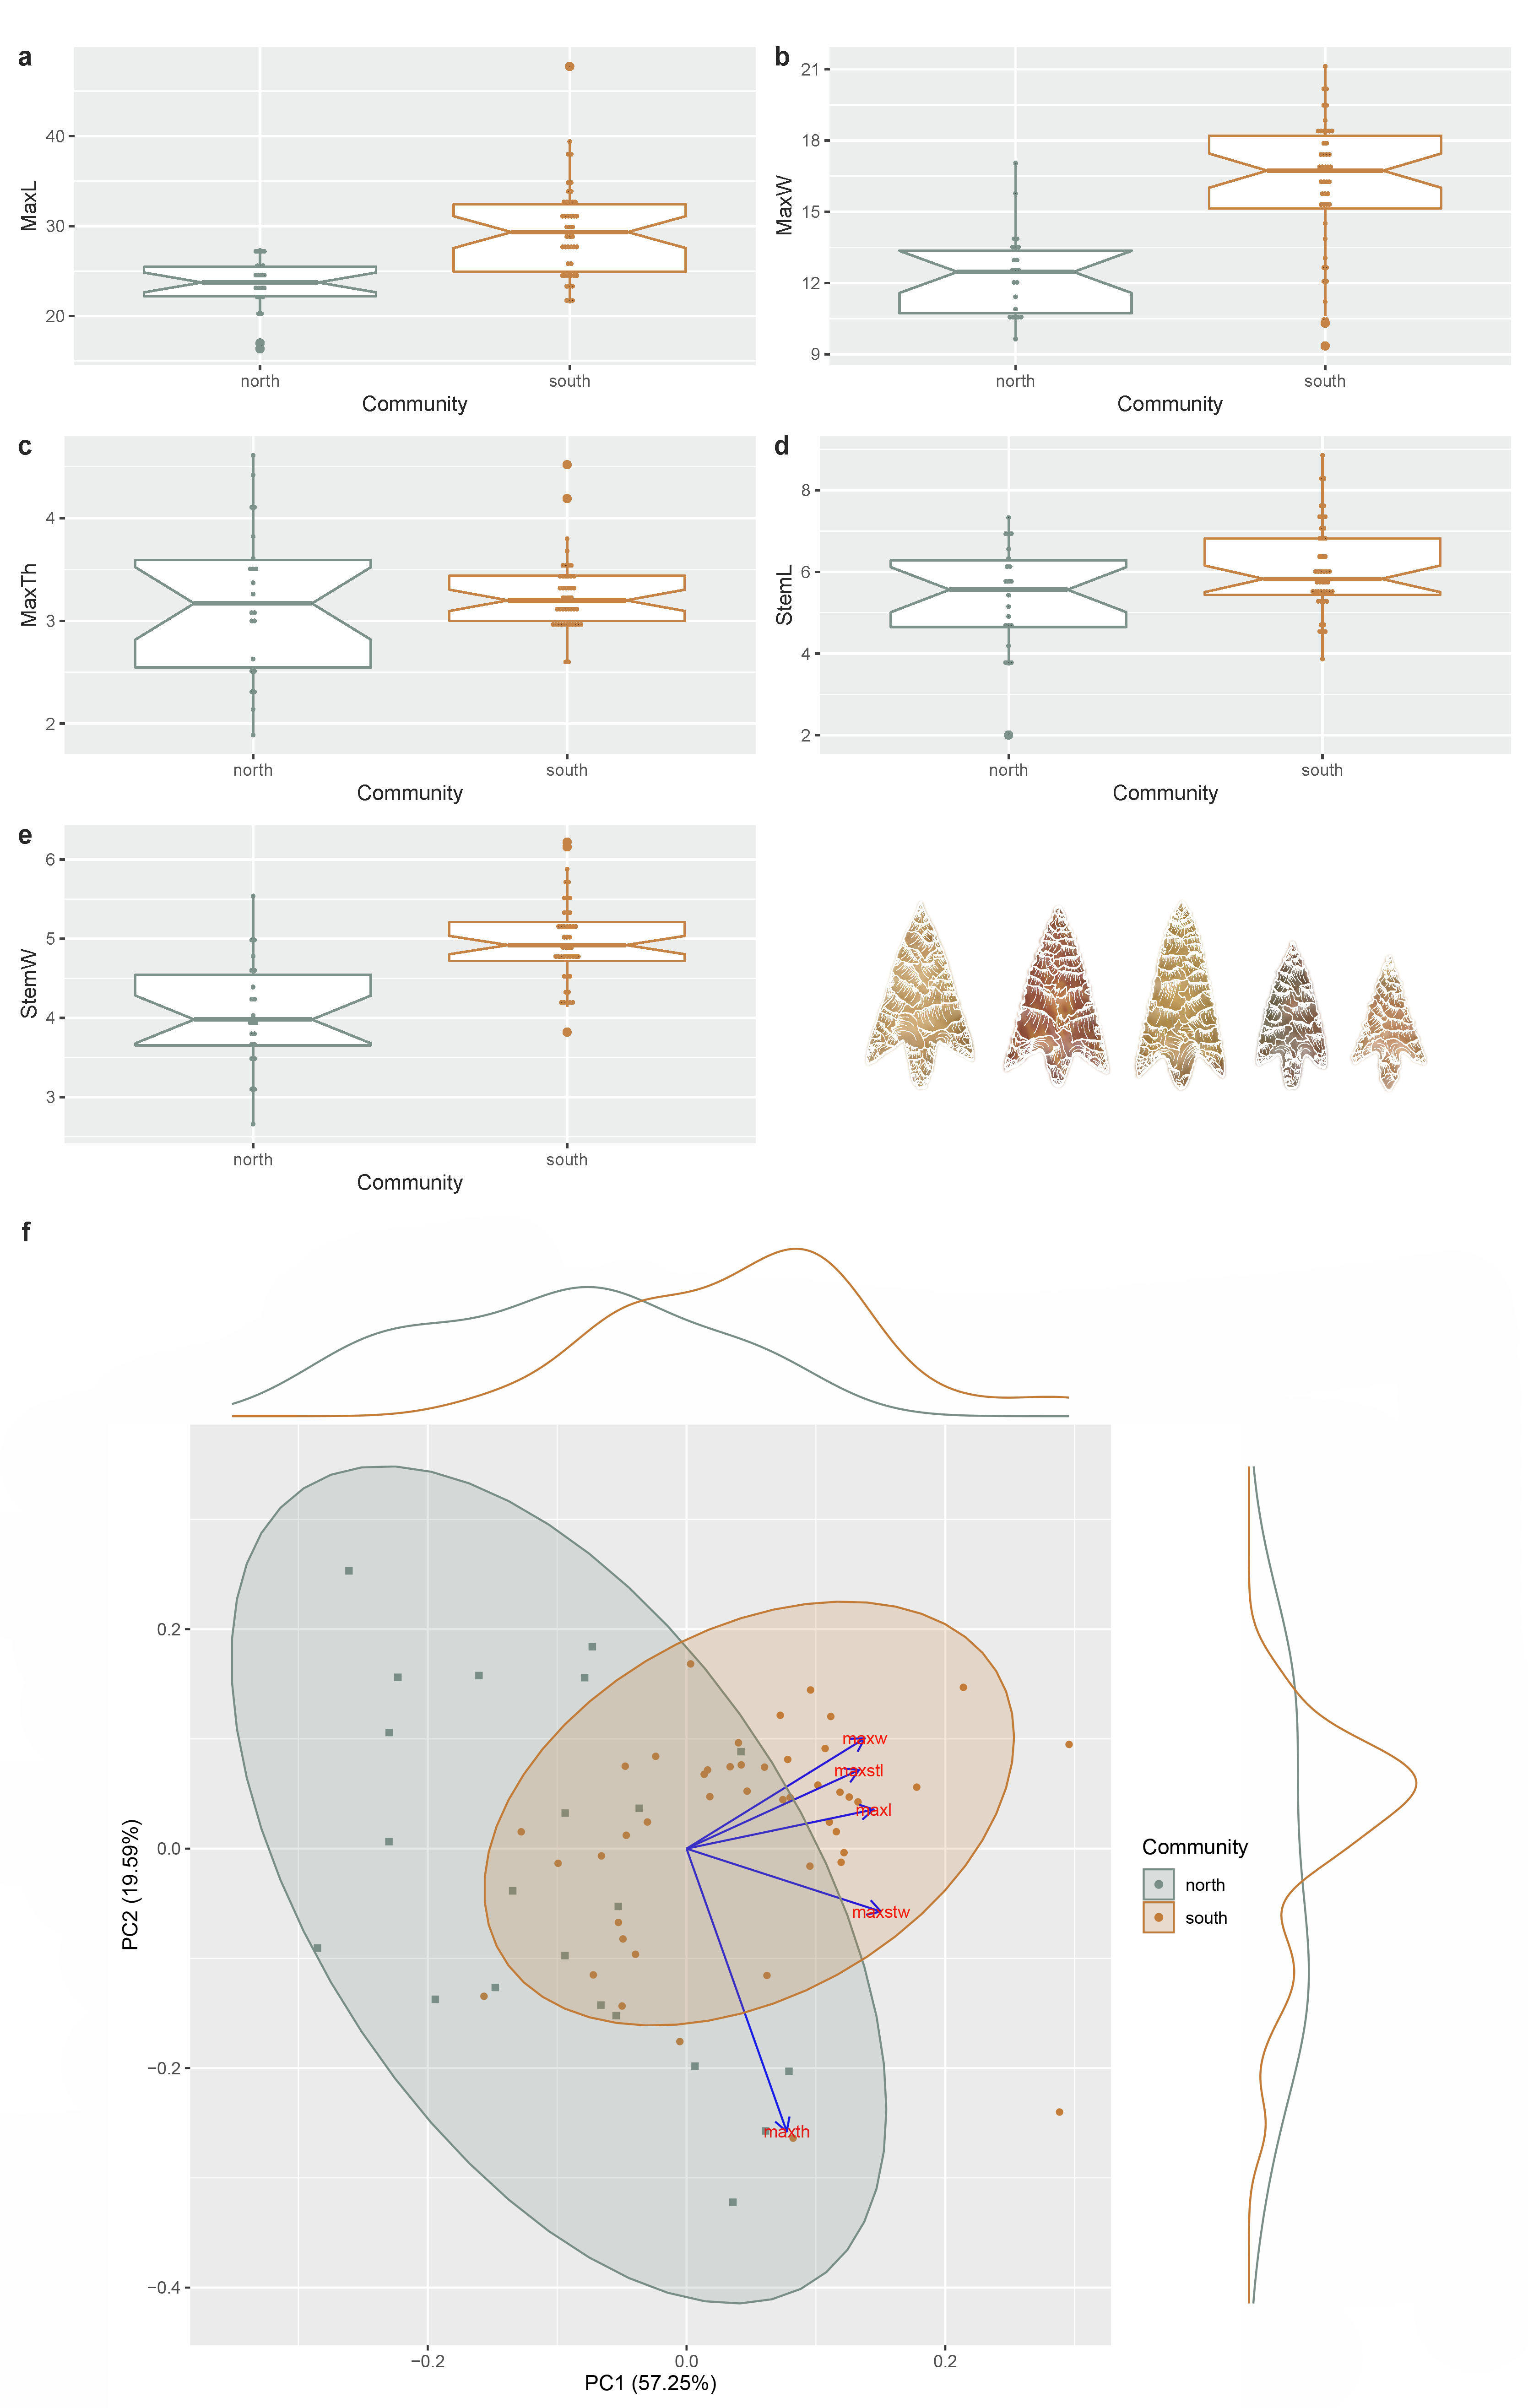
\includegraphics[width=0.95\linewidth]{ms-figs/figure2} \caption{Boxplots for a, maximum length; b, maximum width; c, maximum thickness; d, stem length; e, stem width, and f, PCA [on correlation matrix] for linear metrics associated with the Perdiz arrow points. Additional information related to the analysis, including all linear data and the code needed to reproduce these results, can be found in the supplemental materials at https://seldenlab.github.io/perdiz3/.}\label{fig:fig2}
\end{figure}

\hypertarget{predictive-model}{%
\subsection{Predictive model}\label{predictive-model}}

A \emph{support vector machine} is a supervised machine learning model
regularly used in classifying archaeological materials
\cite{RN9515,RN9516,RN9514,RN9513,RN10755,RN10754}, which has utility in
comparing and classifying datasets aggregated from digital repositories,
comparative collections, open access reports, as well as other digital
assets. For this effort, linear data were imported and modeled using the
\texttt{scikit-learn} package in Python \cite{scikit-learn,sklearn_api}
(\href{https://seldenlab.github.io/perdiz3/}{supplementary materials}),
and subsequently split into training (75 percent) and testing (25
percent) subsets. A standard scaler was used to decrease the sensitivity
of the algorithm to outliers by standardizing features, and a nested
cross validation of the training set was used to achieve unbiased
estimates of model performance, resulting in a mean cross validation
score of 86 percent
(\href{https://seldenlab.github.io/perdiz3/}{supplementary materials}).
The model was subsequently fit on the training set, yielding a receiver
operator curve score of 97 percent, and an accuracy score of 94 percent
(\href{https://seldenlab.github.io/perdiz3/}{supplementary materials}).

\hypertarget{geometric-morphometrics}{%
\subsection{Geometric morphometrics}\label{geometric-morphometrics}}

Each of the arrow points was imaged using a flatbed scanner (HP Scanjet
G4050) at 600 dpi. The landmarking protocol developed for this study
(\href{https://seldenlab.github.io/perdiz3/}{supplementary materials})
included six landmarks and 24 equidistant semilandmarks to characterize
Perdiz arrow point shape, and were applied using the
\texttt{StereoMorph} package in R \cite{RN8973}. The characteristic
points and tangents used in the landmarking protocol were inspired by
the work of Birkhoff \cite{RN5700}.

Landmarks were aligned to a global coordinate system
\cite{RN8102,RN8587,RN8384}, achieved through generalized Procrustes
superimposition \cite{RN8525}, performed in R 4.1.1 \cite{RN8584} using
the \texttt{geomorph} package v4.0.1 \cite{RN8565,RN9565} (Figure
\ref{fig:fig3}). Procrustes superimposition translates, scales, and
rotates the coordinate data allowing for comparisons among objects
\cite{RN5698,RN8525}. The \texttt{geomorph} package uses a partial
Procrustes superimposition that projects the aligned specimens into
tangent space subsequent to alignment in preparation for the use of
multivariate methods that assume linear space \cite{RN8511,RN8384}.

\begin{figure}
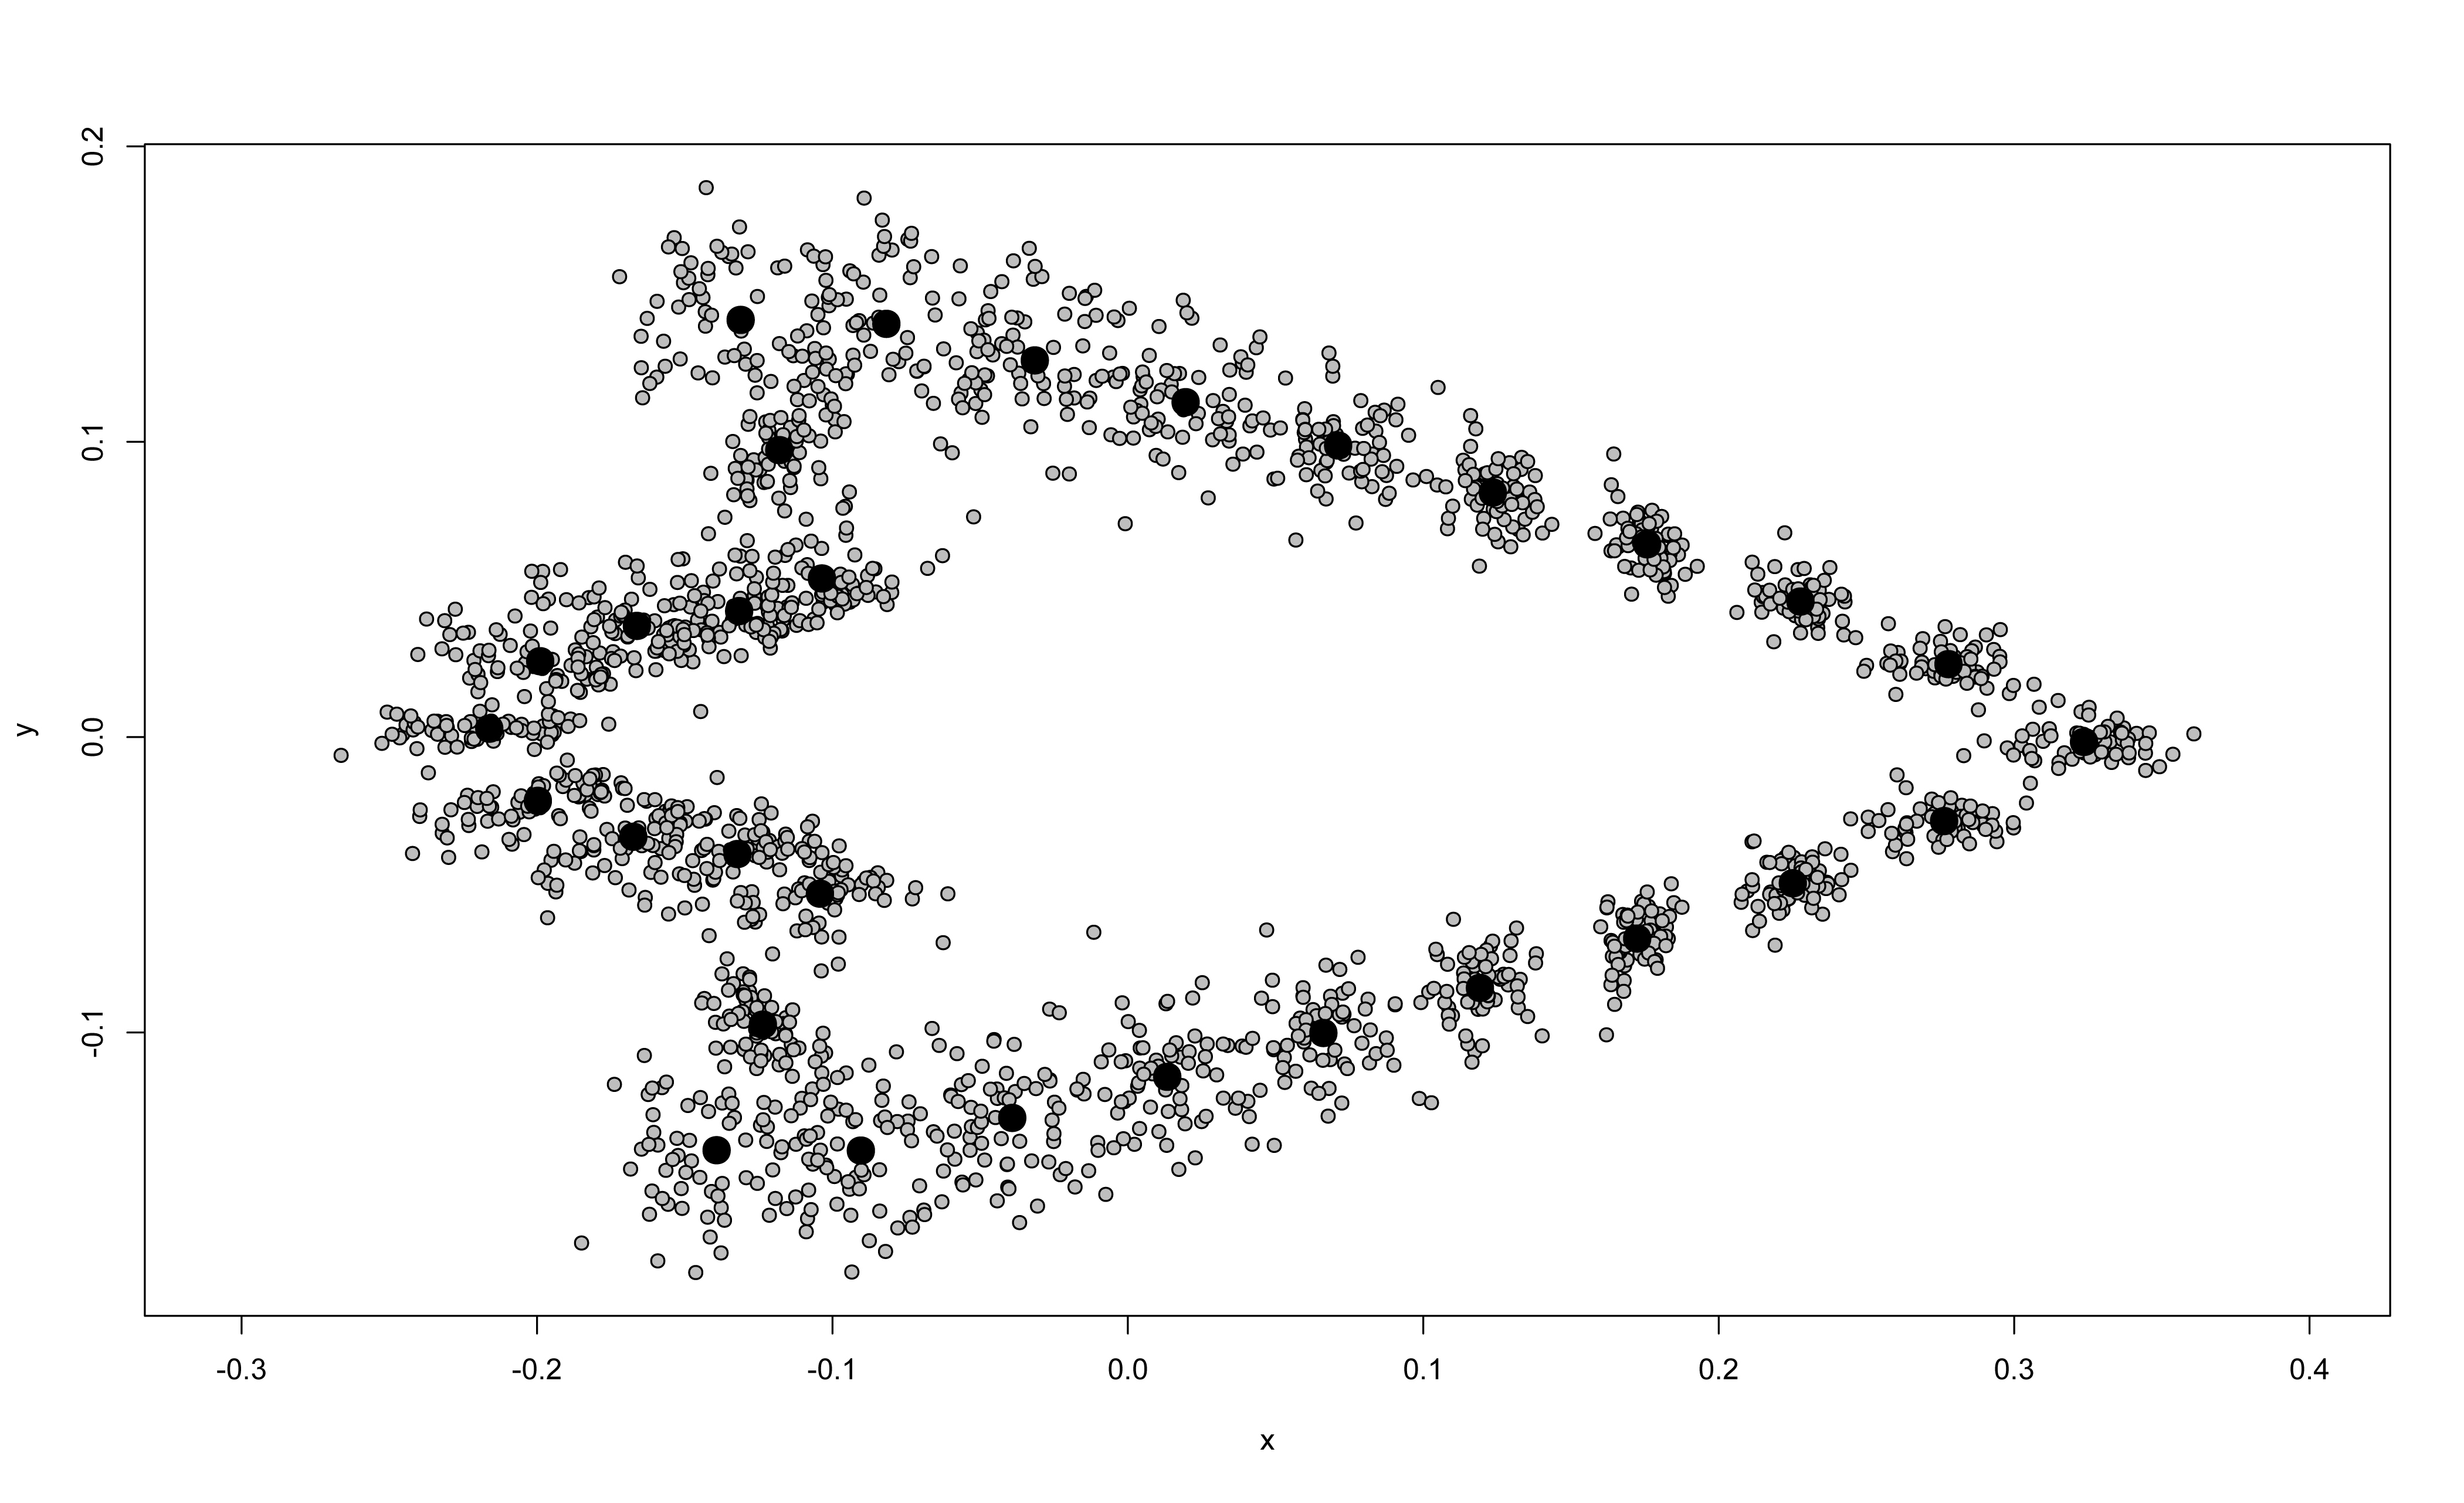
\includegraphics[width=0.95\linewidth]{ms-figs/figure3} \caption{Results of generalized Procrustes analysis, illustrating mean shape (black) and all specimens in the sample (gray), as well as the difference in centroid size for Perdiz arrow points from the two behavioral regions. Additional information related to the GPA, including all data and code needed to reproduce these results, can be found in the supplemental materials at https://seldenlab.github.io/perdiz3/.}\label{fig:fig3}
\end{figure}

Principal components analysis \cite{RN8576,RN10875} was used to
visualize shape variation among the arrow points (Figure
\ref{fig:fig4}). Shape changes described by each principal axis are
commonly visualized using thin-plate spline warping of a reference image
or 3D mesh \cite{RN8555,RN8553}. A residual randomization permutation
procedure (RRPP; n = 10,000 permutations) was used for all Procrustes
ANOVAs \cite{RN8579,RN8334}, which has higher statistical power and a
greater ability to identify patterns in the data should they be present
\cite{RN6995}. To assess whether shape differs by group (region),
Procrustes ANOVAs \cite{RN7046} were also run that enlist effect-sizes
(z-scores) computed as standard deviates of the generated sampling
distributions \cite{RN8477}. Procrustes variance was used to
discriminate between regions and compare the amount of shape variation
(morphological disparity) \cite{RN5703}, estimated as Procrustes
variance using residuals of linear model fit \cite{RN8314}. A pairwise
comparison of morphological integration was used to test the strength of
integration between blade and basal morphology using a z-score
\cite{RN8588,RN8477,RN8340,RN10874}.

\begin{figure}
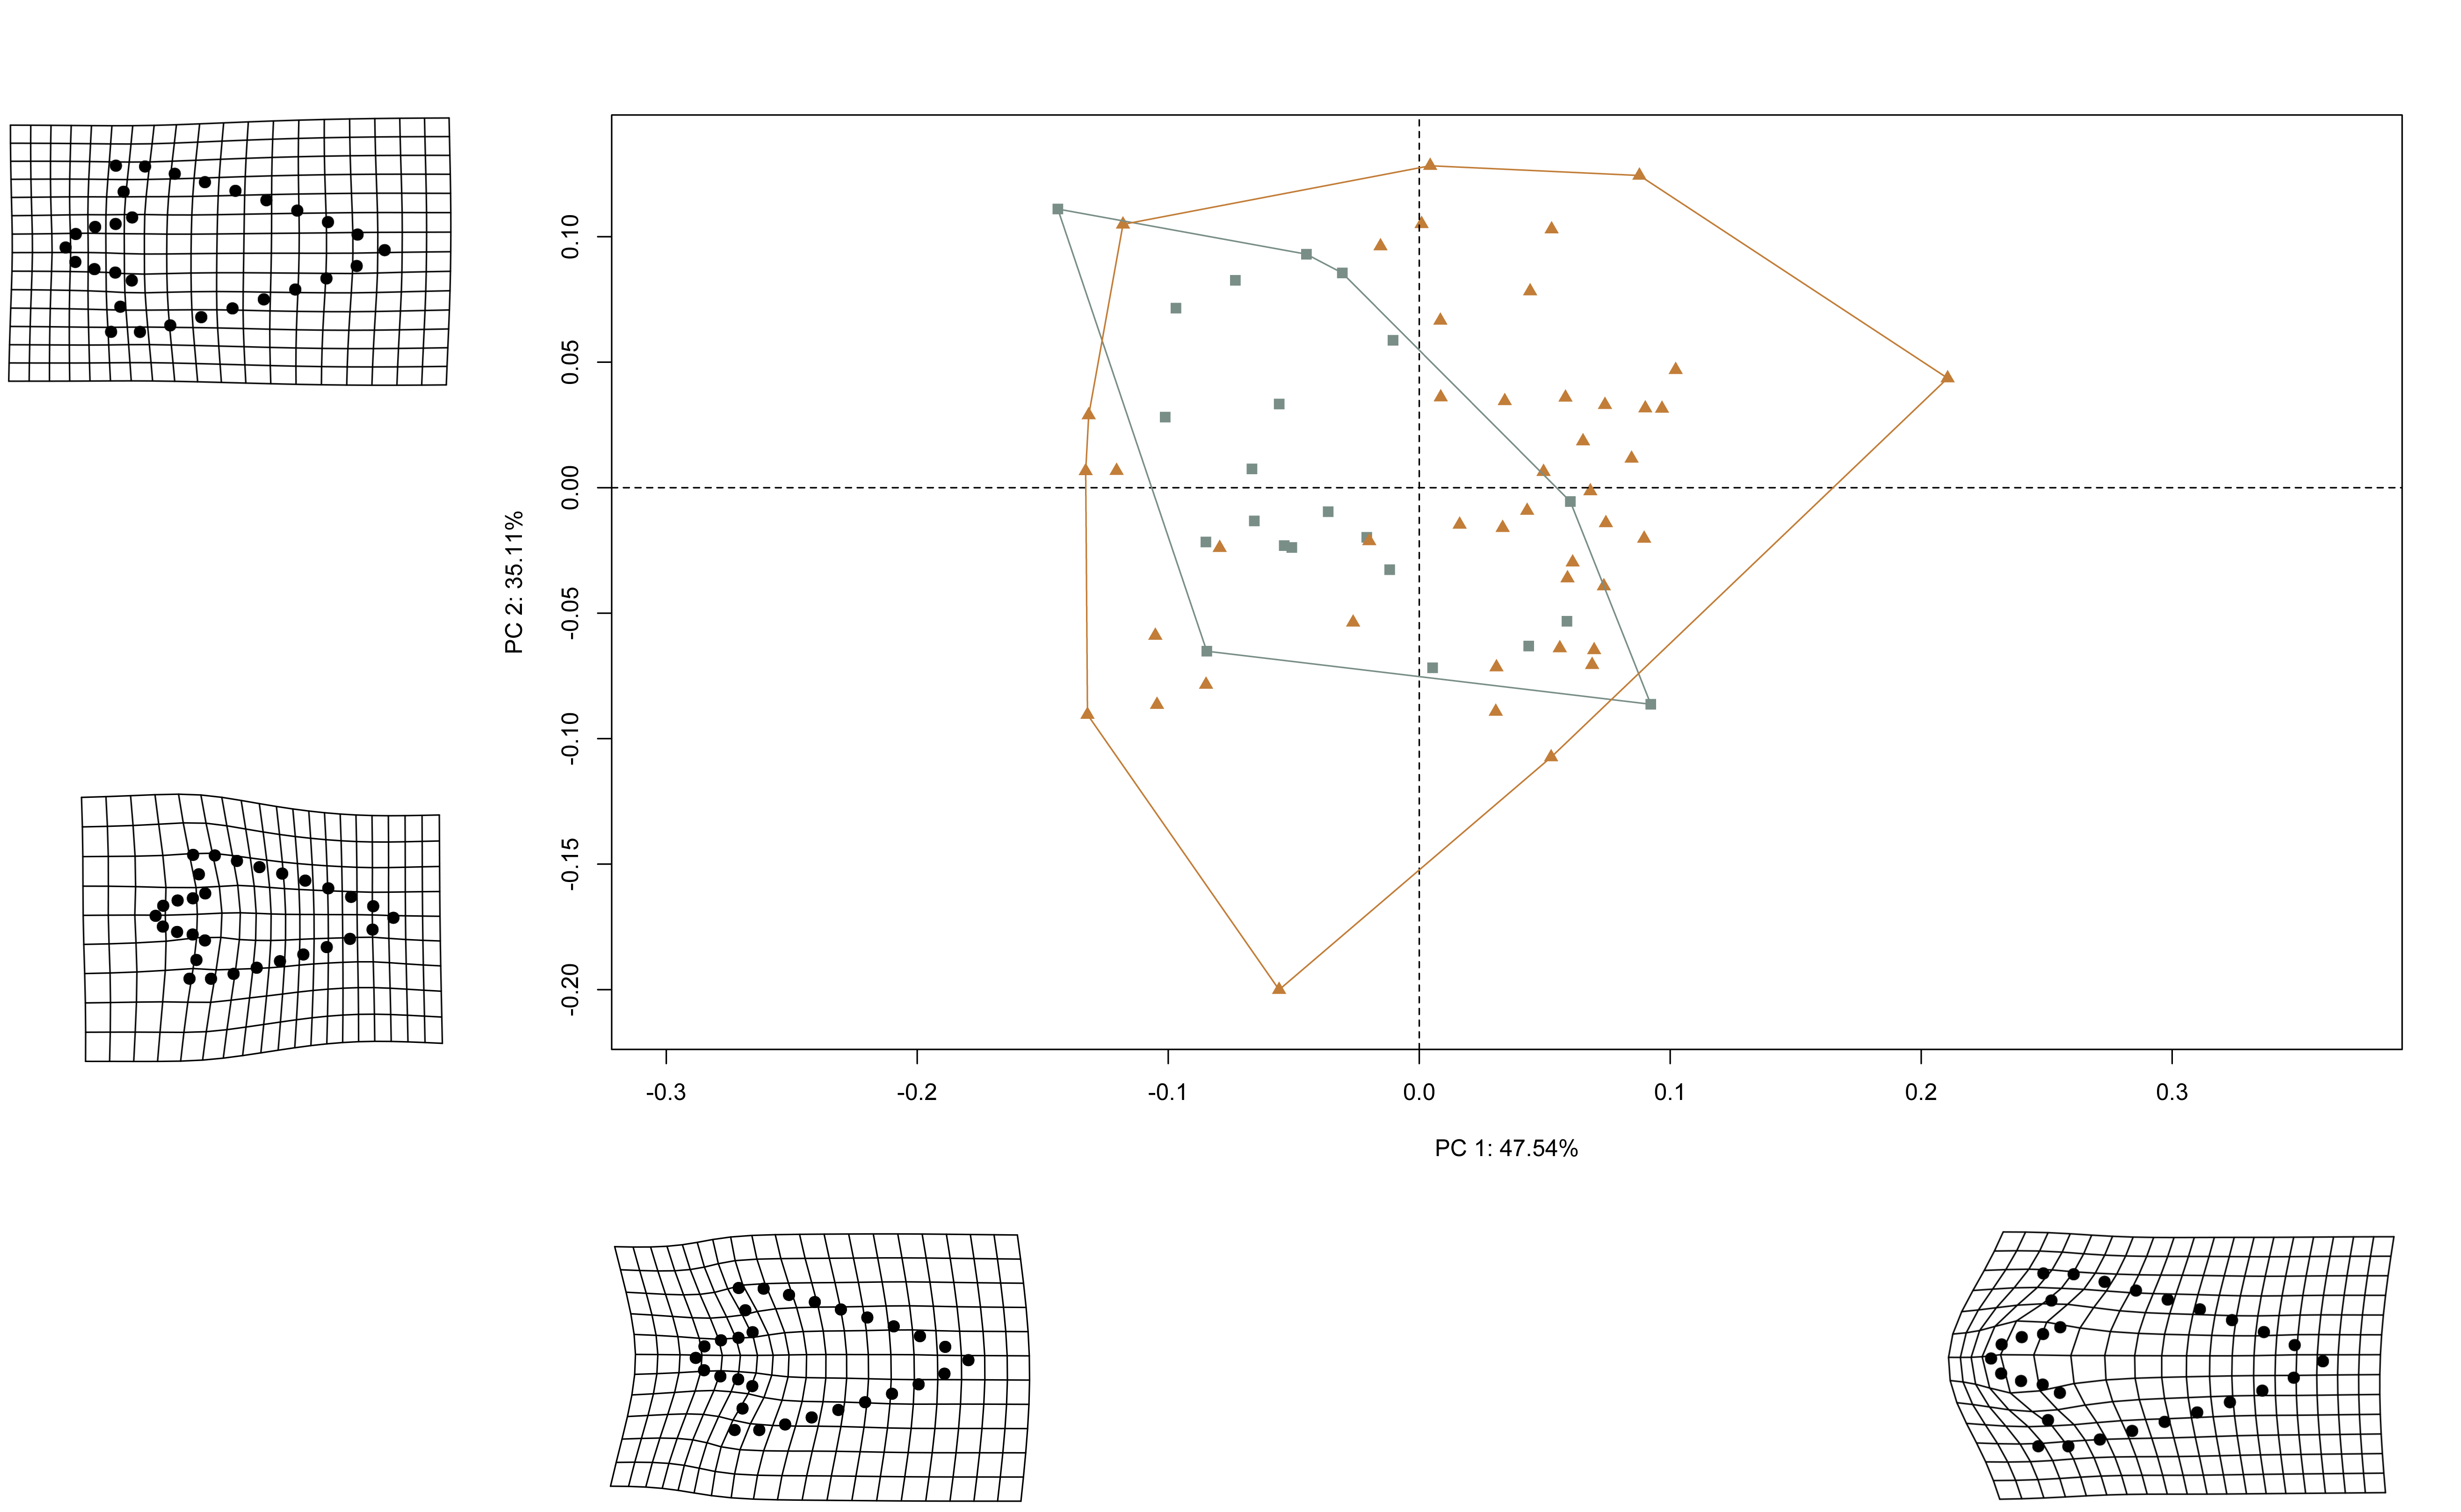
\includegraphics[width=1\linewidth]{ms-figs/figure4} \caption{Principal components analysis plot (PC1/PC2) for Perdiz arrow points by behavioral region/community (top; gray squares, north; orange triangles, south), and results of modularity (bottom left) and blade/base morphological integration (bottom right) analyses. Additional information related to the PCA, including the full listing of results and all data and code needed to reproduce these results, can be found in the supplemental materials at https://seldenlab.github.io/perdiz3/.}\label{fig:fig4}
\end{figure}

A Procrustes ANOVA was used to test for a difference in Perdiz arrow
point (centroid) size by behavioral region (RRPP = 10,000; Rsq =
0.30681; Pr(\textgreater F) = 1e-04), followed by a second to test for a
difference in arrow point shape (RRPP = 10,000; Rsq = 0.0536;
Pr(\textgreater F) = 0.0161). While shape and size differ significantly
between behavioral regions, the Rsq value for size is just under six
times larger than that for shape (smaller in the north; larger in the
south), suggesting that between-region differences in Perdiz arrow point
\emph{size} may be more visually apparent than differences in
\emph{shape}. A comparison of mean consensus configurations was used to
illustrate shape differences from the northern and southern behavioral
regions. Diacritical morphology is characterized by a comparatively
smaller blade and larger stem in the north, and by a comparatively
larger blade and smaller stem in the south. Further, the angle between
the shoulder and base is more acute, with a base that is generally
shorter and narrower in the southern behavioral region
(\href{https://seldenlab.github.io/perdiz3/}{supplementary materials}).

The analysis of modularity, which compares within-module covariation of
landmarks against between-module covariation was significant (see Figure
\ref{fig:fig4} and
\href{https://seldenlab.github.io/perdiz3/}{supplementary materials})
\cite{RN10874,RN5170}, demonstrating that Perdiz arrow point blades and
bases are, in fact, modular. The test for morphological integration was
also significant (see Figure \ref{fig:fig4} and
\href{https://seldenlab.github.io/perdiz3/}{supplementary materials}),
indicating that the blades and bases of Perdiz arrow points are
integrated. These results demonstrate that blade and base shapes for
Perdiz arrow points are predictable; a finding that would have utility
in subsequent studies of Perdiz arrow point morphology that incorporate
fragmentary specimens.

\hypertarget{discussion}{%
\section{Discussion}\label{discussion}}

The shape boundary empirically delineates two discrete behavioral
regions in the ancestral Caddo area. That Perdiz arrow points recovered
from Caddo burials north and south of the shape boundary were found to
differ significantly, expands the scope of the behavioral regions to
include three classes of material culture (Caddo bottles, bifaces,
and---now---arrow points)
\cite{RN8074,RN7927,RN8370,RN8312,RN8322,RN8158,RN11097}. Thus, for
material culture included in burial contexts north and south of the
shape boundary, the Caddo were selecting for significant morphological
differences in bottles, bifaces, and arrow points (Figure
\ref{fig:fig6}a-d). Results clearly illustrate that morphological
differences among Perdiz arrow points found in the northern and southern
behavioral regions (Figure \ref{fig:fig6}d) are predictable
(\href{https://seldenlab.github.io/perdiz3/}{supplementary materials}),
and can be disaggregated using a standard suite of linear metrics
regularly collected in the course of cultural resource management
endeavors.

\begin{figure}
\includegraphics[width=1\linewidth]{ms-figs/figure6} \caption{Mean shapes and comparisons for a, Formative/Early and b, Late/Historic bottles; c, Formative/Early Gahagan bifaces; and d, Middle/Late Perdiz arrow points from Caddo burial contexts in the northern and southern behavioral regions. In the comparisons of mean shape, the northern population appears in gray, and the southern population appears in black.}\label{fig:fig6}
\end{figure}

The geometric morphometric analysis demonstrated significant
morphological differences for Perdiz arrow points recovered north and
south of the shape boundary, where the most pronounced difference was
found to occur in basal morphology (see Figure \ref{fig:fig6}d). This
finding provides evidence in support of the argument that Perdiz arrow
point morphology is labile \cite{RN9364}. The character of those
morphological differences found to occur in Perdiz arrow points (basal
morphology and size) is potentially suggestive of differential
approaches to hafting.

Blades and bases of Perdiz arrow points were found to be both modular
and morphologically integrated. This indicates that each module
functions independently, and that basal shape is a predictor of blade
shape, and vice-versa. Further work is warranted to assess whether
Perdiz arrow points from groups within the boundaries of the northern
and southern behavioral regions may express unique morphologies, aiding
in further delimiting local boundaries associated with constituent Caddo
groups.

\hypertarget{morphologically-distinct-behavioral-regions}{%
\subsection{Morphologically-distinct behavioral
regions}\label{morphologically-distinct-behavioral-regions}}

In considering the role/s of material culture as aspects of social
identity, it is important not to lose sight of the fact that people and
their possessions are active agents in the production and maintenance of
social identity/ies. All three categories of material culture (bottles,
bifaces, and arrow points) contribute to local and regional communities
of identity and communities of practice \cite{RN8061}. Generally, this
concept may be more easily applied to bottles since those were
manufactured and used by individuals sharing collective Caddo
identities. Bifaces and arrow points potentially represent multiple
identities---those being the Caddo, as users; and non-Caddo, as
producers---at least with regard to chipped stone tools incorporated in
mortuary contexts. This concept lends defensible credence to the notion
of morphologically-distinct behavioral regions among the Caddo, while
integrating the possibility of understanding interactions between Caddo
and non-Caddo groups, to include the movement of material culture
between Caddo behavioral regions.

Three categories of Caddo material culture have been demonstrated to
differ north and south of the shape boundary, indicating a haecceity of
regional perspectives related to production (bottles), and aesthetic
choice/cultural interaction (bifaces and arrow points). These differing
perspectives incorporate normative group decisions that include shape,
size, form, and decorative expression, which likely represent the
culmination of generational perspectives \cite{RN5610}. Simply stated,
such perspectives are representative of tradition. Eckert and colleagues
\cite{RN8061} indicate that provenance, the origin or source of an item,
is a significant component of understanding the interrelatedness of
communities of identity and communities of practice. A second shape
boundary demonstrates that Gahagan bifaces differ significantly between
the ancestral Caddo region and central Texas, where they are currently
thought to have been manufactured. This suggests that those communities
of practice that articulate with the \emph{production} of chipped stone
artifacts recovered from Caddo internments, may not have been Caddo.

It is also entirely possible that there are no communities of practice
for chipped stone artifacts recovered from Caddo mortuary contexts.
However, there do appear to have been communities of practice associated
with Perdiz arrow points recovered from non-mortuary contexts in the
ancestral Caddo area, which may more readily reflect retouch or
resharpening approaches used by Caddo knappers
\cite{RN9364,RN8486,RN11097}. Similar interpretations can be applied to
the Gahagan bifaces, as few have been reported outside of Caddo mortuary
contexts. It may be more fitting to perceive of Perdiz arrow points and
Gahagan bifaces as indicative of communities of identity rather than
communities of practice, due to the contextual discrepancy evinced
through mortuary and non-mortuary settings. The provenance of bifaces
from Caddo mortuary contexts can most assuredly be considered non-local,
or produced outside of the ancestral Caddo region, based on multiple
factors that include raw material, workmanship, morphology, and context.

\hypertarget{conclusion}{%
\section{Conclusion}\label{conclusion}}

This study demonstrated that linear metrics and shape variables
collected for Perdiz arrow points support the shape boundary posited in
recent social network and geometric morphometric analyses, and
determined that those same metrics can be used to predict regional
membership. Morphological features that discriminate between Perdiz
arrow points recovered from each behavioral region were identified using
geometric morphometrics, with substantive differences found to occur in
size and basal morphology. Blade and base shape were found to be both
modular and morphologically integrated, suggesting that blade and base
shapes are predictable. While evidence from one category---Caddo
bottles---supports discussions of Caddo production, the other
two---bifaces and arrow points---may articulate with production
activities outside of the region by non-Caddo makers. Such production
activity is more likely to be localized than exchange systems, thus
assumed to leave a clearer signature \cite{RN7019}.

\hypertarget{acknowledgments}{%
\section*{Acknowledgments}\label{acknowledgments}}
\addcontentsline{toc}{section}{Acknowledgments}

We extend our gratitude to the Caddo Nation of Oklahoma, the Caddo
Nation Tribal Council, Tribal Chairman, and Tribal Historic Preservation
Office for their continued guidance and support of our work, as well as
access to NAGPRA and previously repatriated collections. Thanks also to
the Anthropology and Archaeology Laboratory at Stephen F. Austin State
University for the requisite permissions and access to the NAGPRA
objects from the Washington Square Mound site and Turner collections,
and to Tom A. Middlebrook for brokering access to the Perdiz arrow
points from burials at the Morse Mound site. We wish to thank Michael J.
Shott and Casey Wayne Riggs for their useful comments and constructive
criticisms on a presubmission draft, and extend our gratitude to Emma
Sherratt, Kersten Bergstrom, Lauren Butaric, Julien Claude, Dean C.
Adams, and Michael L. Collyer for their constructive criticisms and
suggestions throughout the development of this research program.
Additional comments from the editor and three anonymous reviewers aided
in further refining the manuscript.

\hypertarget{funding}{%
\section*{Funding}\label{funding}}
\addcontentsline{toc}{section}{Funding}

Components of the analytical workflow were developed and funded by a
Preservation Technology and Training grant (P14AP00138) to RZS from the
National Center for Preservation Technology and Training, as well as
grants to RZS from the Caddo Nation of Oklahoma, National Forests and
Grasslands in Texas (15-PA-11081300-033) and the United States Forest
Service (20-PA-11081300-074). Additional funding and logistical support
was provided by the Heritage Research Center at Stephen F. Austin State
University.

\hypertarget{data-management}{%
\section*{Data Management}\label{data-management}}
\addcontentsline{toc}{section}{Data Management}

The data and analysis code associated with this project can be accessed
through the GitHub repository
(\url{https://github.com/seldenlab/perdiz3}) or the supplementary
materials (\url{https://seldenlab.github.io/perdiz3/}); which are
digitally curated on the Open Science Framework \newline 
(\href{https://osf.io/vzhjr/}{DOI: 10.17605/OSF.IO/VZHJR}). Images of
all Perdiz arrow points used in this study were made available in an
open access comparative collection
(\url{https://scholarworks.sfasu.edu/ita-perdiz/}), with permission from
the Caddo Nation of Oklahoma. These supplementary materials include all
analysis data and code used in the study, providing a means for others
to reproduce (exactly) those results discussed and expounded upon in
this article. The replicable nature of this undertaking provides others
with the means to critically assess and evaluate the various analytical
components of this study, which is a necessary requirement for the
production of reliable knowledge \cite{RN20915,RN20916,RN20917}.

Reproducibility projects in \href{https://osf.io/ezcuj/}{psychology} and
\href{https://www.cos.io/rpcb}{cancer biology} are impacting current
research practices across all domains. Examples of reproducible research
are becoming more abundant in archaeology
\cite{RN20804,RN21009,RN8322,RN9364,RN11097}, and the next generation of
archaeologists are learning those tools and methods needed to reproduce
and/or replicate research results \cite{RN21007}. Reproducible and
replicable research work flows are often employed at the highest levels
of humanities-based inquiries to mitigate concern or doubt regarding
proper execution, and is of particular import should the results
have---explicitly or implicitly---a major impact on scientific progress
\cite{RN21008}.


\bibliographystyle{spmpsci}
\bibliography{mybibfile.bib}


\end{document}
